% Don't forget to compile TWICE so the refernces are correct.

% When you start writing a talk by renaming this template, consider the following:  
%
%A common temptation for first-time slide makers is to name it something like ``my_talk.tex'' or ``john_doe_talk.tex'' or even ``discrete_math_seminar_talk.tex''.  You really won't like any of these titles the second time you give a talk.  Try naming your tex file something more descriptive, like ``riemann_hypothesis_short_proof_talk.tex''.  Even better (in case you recycle 99% of a talk, but still want to change a little, and retain copies of each), how about ``riemann_hypothesis_short_proof_MIT-Colloquium.2000-01-01.tex''?


%%%%%%%%%%%%%%
% BASIC FORMATTING %
%%%%%%%%%%%%%%

\documentclass[notes, compressed, blue]{beamer}

%LOAD VARIOUS PACKAGES
\usepackage{amsmath,amssymb,amsthm,amsfonts,graphicx,url,colordvi}
\usepackage{graphics,graphics,latexsym,multicol,epsfig}
\usepackage{enumerate,url,multimedia}
\usepackage{verbatim}

%%%%%%%%%%%%%%%%%%%%
% BUILD YOUR OWN SHORTCUTS %
%%%%%%%%%%%%%%%%%%%%


%MATH CHARACTER COMMANDS
\newcommand{\R}{\mathbb R} %REALS
\newcommand{\C}{\mathbb C} %COMPLEX
\newcommand{\N}{\mathbb N} %NATURAL NUMBERS
\newcommand{\Q}{\mathbb Q} %RATIONALS
\newcommand{\Z}{\mathbb Z} %INTEGERS

%LOWER CASE VECTORS v, x, AND b IN BOLDFACE
\newcommand{\vecv}{\mathbf v} 
\newcommand{\vecx}{\mathbf x}
\newcommand{\vecb}{\mathbf b}

%SYMBOL TAU IN BOLD
\newcommand{\tor}{\boldsymbol{\tau}}

%FORMAT THEOREMS
%\newtheorem{theorem}{Theorem}[section]
%\newtheorem{lemma}[theorem]{Lemma}
\newtheorem{conjecture}[theorem]{Conjecture}
\newtheorem{problemma}[theorem]{Problemma}
\newtheorem{proposition}[theorem]{Proposition}
%\newtheorem{definition}[theorem]{Definition}
%\newtheorem{corollary}[theorem]{Corollary}
\newtheorem{remark}[theorem]{Remark}
%\newtheorem{example}[theorem]{Example}
\newtheorem{claim}{Claim}

%DEFINE NEW NAMED FUNCTIONS
\DeclareMathOperator{\rank}{rank}
\DeclareMathOperator{\Hom}{Hom}
\DeclareMathOperator{\conv}{conv}


%%%%%%%%%%%%%%%%
% MATH  ENVIRONMENTS %
%%%%%%%%%%%%%%%%


%INLINE EQUATION
% $f(x) = x^2$
% $\displaystyle f(x)=x^2$

%CENTERED EQUATION
% $$ f(x)=x^2 $$

%LABELED EQUATION. 
%(TO REFER TO THE EQUATION LATER IN TEXT TYPE "(\ref{quadratic})".)
%begin{equation}\label{quadratic}
% f(x)=x^2
%\end{equation}

%ALIGNED FORMULA WITHOUT LABELLING
%\begin{align*}
%f(x)&=x^2-2x+1 \\
%   &=(x-1)^2 \\
% 	&< 5.
%\end{align*}


%%%%%%%%%
% EXAMPLES %
%%%%%%%%%
 

%1. FRACTIONS AND RADICALS

% $\frac{x-1}{x+1}$
% $\sqrt[n]{x^2+1}$ 

%2. MATRIX COMMANDS

% $\begin{matrix}a & b \\ c & d \end{matrix}$
% $\begin{bmatrix}a & b \\ c & d \end{bmatrix}$
% $\begin{pmatrix}a & b \\ c & d \end{pmatrix}$

%3. INTEGRAL

% $\int_{x=0}{x=1}x^2 \ dx$

%4. PIECEWISE DEFINED FUNCTION

% $p(t)=\begin{cases} \frac{1}{2}, &\text{if $t \in [-1,1]$}; \\ 0, &\text{otherwise,} \end{cases}$


%%%%%%%%%%%%%%%
% FIGURES AND TABLES %
%%%%%%%%%%%%%%%


%FIGURES

%\begin{figure}[h]
%\hfil \scalebox{.5}{ \rotatebox{0}{ \includegraphics{c:/images/sampleimage.eps} }}  \hfil 
%\caption{ Sample figure }
%\end{figure}

%TABLE COMMANDS 

%\begin{tabular}{c|c} $x$ & $y$ \\ \hline a & b \\ c & d \\ e & f \ \end{tabular}

%MULTICOLUMN TABLE

%\begin{table}[h]
%\begin{center}
%\begin{tabular}{|c|c|c|c|c|c|c|} 
%\hline
%& \multicolumn{6}{c|}{Genotype of Parents}\\ \hline
%Genotype of Offspring & AA-AA & AA-Aa & AA-aa & Aa-Aa & Aa-aa & aa-aa \\ \hline 
%AA &  &  &  & &  &    \\ \hline
%Aa &  &  &  & &  &    \\ \hline
%aa &  &  &  & &  &    \\ \hline
%\end{tabular}
%\end{center}
%\end{table}


%%%%%%%%%%%%%
%  MISCELLANEOUS  %
%%%%%%%%%%%%%

  
%WEB URL
%\texttt{http://www.phy.syr.edu/courses/java-suite/crosspro.html} 

%TWO ALIGNED FORMULA COLUMNS
%\begin{alignat}{2}
%P_0(x)&=1, & \qquad P_1(x)&=x \notag \\
%P_2(x)&=\frac{1}{2}(3x^2-1), & \qquad P_3(x)&=\frac{1}{2}(5x^3-3x) \notag 
 % \end{alignat} 

%VARIABLE SPACED COLUMNS IN A TABLE
%\begin{tabular}{p{2.5in} p{2.5in}}
%	$\det(BA)$ &   $\det(A^{-1})$ \vspace{2in} \\
%	$\det(3B)$ &   $\displaystyle \det \left( \begin{bmatrix} 1 & 2 & 4 \\ 2 & 0 & -2 \\ 1 & 2 & 2 \end{bmatrix} \right)$ 
%	\end{tabular}


%%%%%%%%%%%%%%%%%
% PRESENTATION THEMES %
%%%%%%%%%%%%%%%%%

\mode<presentation>
{
  % A tip: pick a theme you like first, and THEN modify the color theme, and then add math content.
  % Warsaw is the theme selected by default in Beamer's installation sample files.

  %%%%%%%%%%%%%%%%%%%%%%%%%%%% THEME
  %\usetheme{AnnArbor}
  %\usetheme{Antibes}
  %\usetheme{Bergen}
  %\usetheme{Berkeley}
  %\usetheme{Berlin}
  %\usetheme{Boadilla}
  %\usetheme{boxes}
  \usetheme{CambridgeUS}
  %\usetheme{Copenhagen}
  %\usetheme{Darmstadt}
  %\usetheme{default}
  %\usetheme{Dresden}
  %\usetheme{Frankfurt}
  %\usetheme{Goettingen}
  %\usetheme{Hannover}
  %\usetheme{Ilmenau}
  %\usetheme{JuanLesPins}
  %\usetheme{Luebeck}
  %\usetheme{Madrid}
  %\usetheme{Malmoe}
  %\usetheme{Marburg}
  %\usetheme{Montpellier}
  %\usetheme{PaloAlto}
  %\usetheme{Pittsburgh}
  %\usetheme{Rochester}
  %\usetheme{Singapore}
  %\usetheme{Szeged}
  %\usetheme{Warsaw}

  %%%%%%%%%%%%%%%%%%%%%%%%%%%% COLOR THEME
  %\usecolortheme{albatross}
  %\usecolortheme{beetle}
  %\usecolortheme{crane}
 \usecolortheme{default}
  %\usecolortheme{dolphin}
  %\usecolortheme{dove}
  %\usecolortheme{fly}
  %\usecolortheme{lily}
  %\usecolortheme{orchid}
  %\usecolortheme{rose}
  %\usecolortheme{seagull}
  %\usecolortheme{seahorse}
  %\usecolortheme{sidebartab}
  %\usecolortheme{structure}
  %\usecolortheme{whale}

  %%%%%%%%%%%%%%%%%%%%%%%%%%%% OUTER THEME
  %\useoutertheme{default}
  %\useoutertheme{infolines}
  %\useoutertheme{miniframes}
  %\useoutertheme{shadow}
  %\useoutertheme{sidebar}
  %\useoutertheme{smoothbars}
  %\useoutertheme{smoothtree}
  %\useoutertheme{split}
  %\useoutertheme{tree}

  %%%%%%%%%%%%%%%%%%%%%%%%%%%% INNER THEME
  %\useinnertheme{circles}
  %\useinnertheme{default}
  %\useinnertheme{inmargin}
  %\useinnertheme{rectangles}
  %\useinnertheme{rounded}

  %%%%%%%%%%%%%%%%%%%%%%%%%%%%%%%%%%%

  \setbeamercovered{transparent} % or whatever (possibly just delete it)
  % To change behavior of \uncover from graying out to totally invisible, can change \setbeamercovered to invisible instead of transparent. apparently there are also 'dynamic' modes that make the amount of graying depend on how long it'll take until the thing is uncovered.
}

\beamertemplatenavigationsymbolsempty  % Get rid of nav bar


% Insert frame number at bottom of the page.
\usefoottemplate{ \hfil \tiny {\color{black} \insertframenumber} } 

\usepackage[english]{babel}
\usepackage[latin1]{inputenc}
\usepackage{times}
\usepackage[T1]{fontenc}
\usepackage{array}
\usepackage{wrapfig}
%%%%%%%%%%%%%%%
% START OF DOCUMENT %
%%%%%%%%%%%%%%%

\title{Correlating Temperature Variation with Phase Noise on LOT}
\author{Sam Tay}
\institute{Astroparticule et Cosmologie}
\date{August 2, 2011}
\subject{Summer Research Project}

\begin{document}



\begin{frame}
  \titlepage
\end{frame}

%\begin{frame}
 % \frametitle{Outline}
  %\tableofcontents
%\end{frame}


\section{An Optical Simulator for LISA}

\begin{frame}
\frametitle{LISA}

LISA (Laser Interferometer Space Antenna) is a space project designed to detect gravitational waves.\\
%\vspace{1cm}
\hspace{.5cm}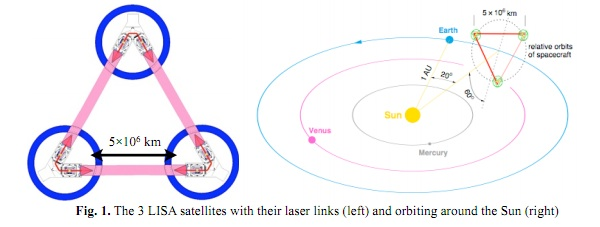
\includegraphics[width=4in]{figure1.jpg}\\
LISA has two main technical difficulties:
\begin{itemize}
\item the free falling masses must be isolated from all forces other than gravity, and the spacecraft must precisely follow these test masses
\item outstanding precision of phase shift measurements.
\end{itemize}
\end{frame}



\begin{frame}
\frametitle{Motivation}

LISA's capability to measure very small displacements relies on a number of algorithms and stabilization techniques, very low noise, and extremely high performance instruments.\\
\vspace{.3cm}
Simulation software can simulate Doppler effects, propogation delays, reconstruction algorithms, etc., and many of the stabilization techniques (such as TDI and arm-locking) have been tested theoretically and by numerical simulation.\\
\vspace{.3cm}
LISA On Table (LOT) is an optical simulator for LISA. This hardware development is desirable in order to characterize detection devices, validate numerical models, and study the influence of the hardware on the detection algorithm.

\end{frame}



\begin{frame}
\frametitle{Experimental Set-up}

\begin{center}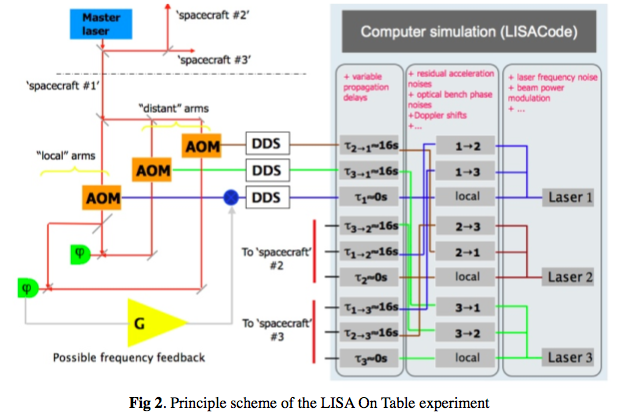
\includegraphics[width=4in]{principle.png}\end{center}

\end{frame}



\begin{frame}
\frametitle{Actual Optomechanical Set-up}

\begin{center}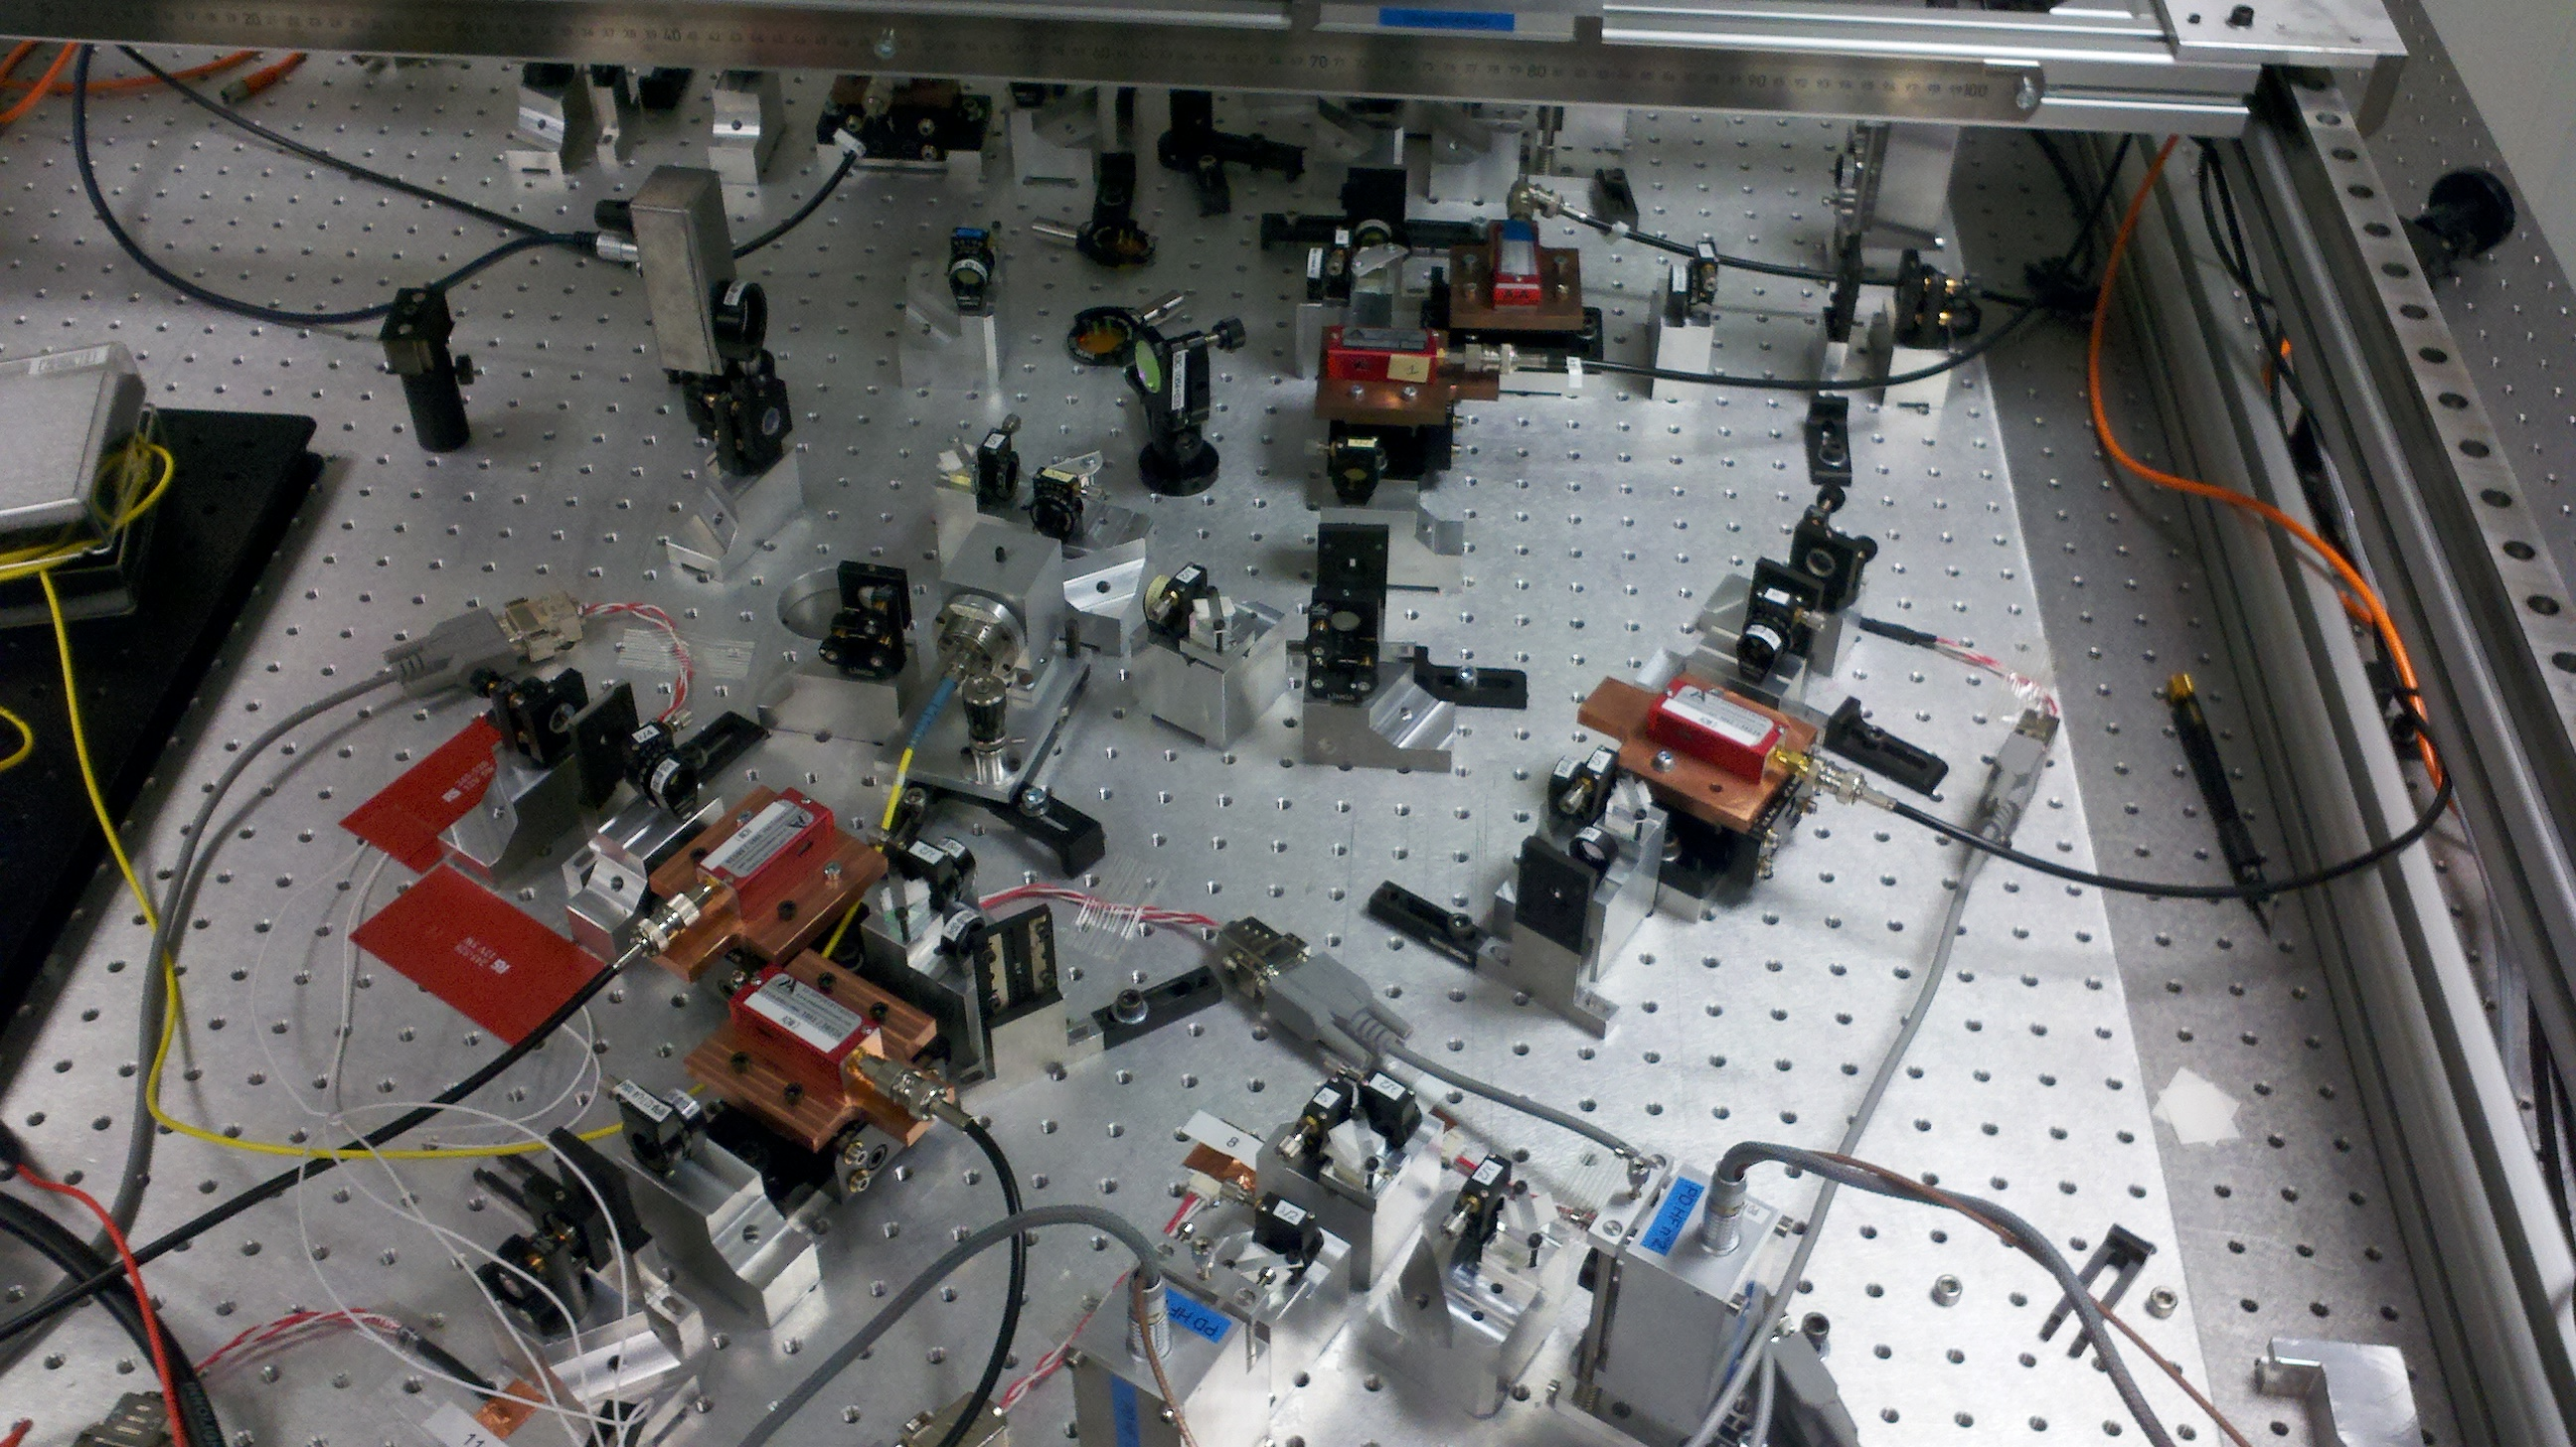
\includegraphics[width=3.6in]{optomechanical.jpg}\end{center}

\begin{itemize}
\item{AOMs are in cat's eye configuration, allowing frequency change with over 20MHz range with small angular deviation}
%\item{AOMs are driven at 110 MHz from DDSs (double pass of configuration results in 220MHz frequency shift)}
\item{Configuration allows two distant beams to follow the same optical path on perpendicular polarizations}
\end{itemize}

\end{frame}





\section{Correlating Phase Noise with Temperature Variation}


\begin{frame}
\frametitle{Expectations}

%EDIT PICTURE TO LOCATE SENSORS AND ARMS%%%%%%%%%%%%%%
    \begin{center}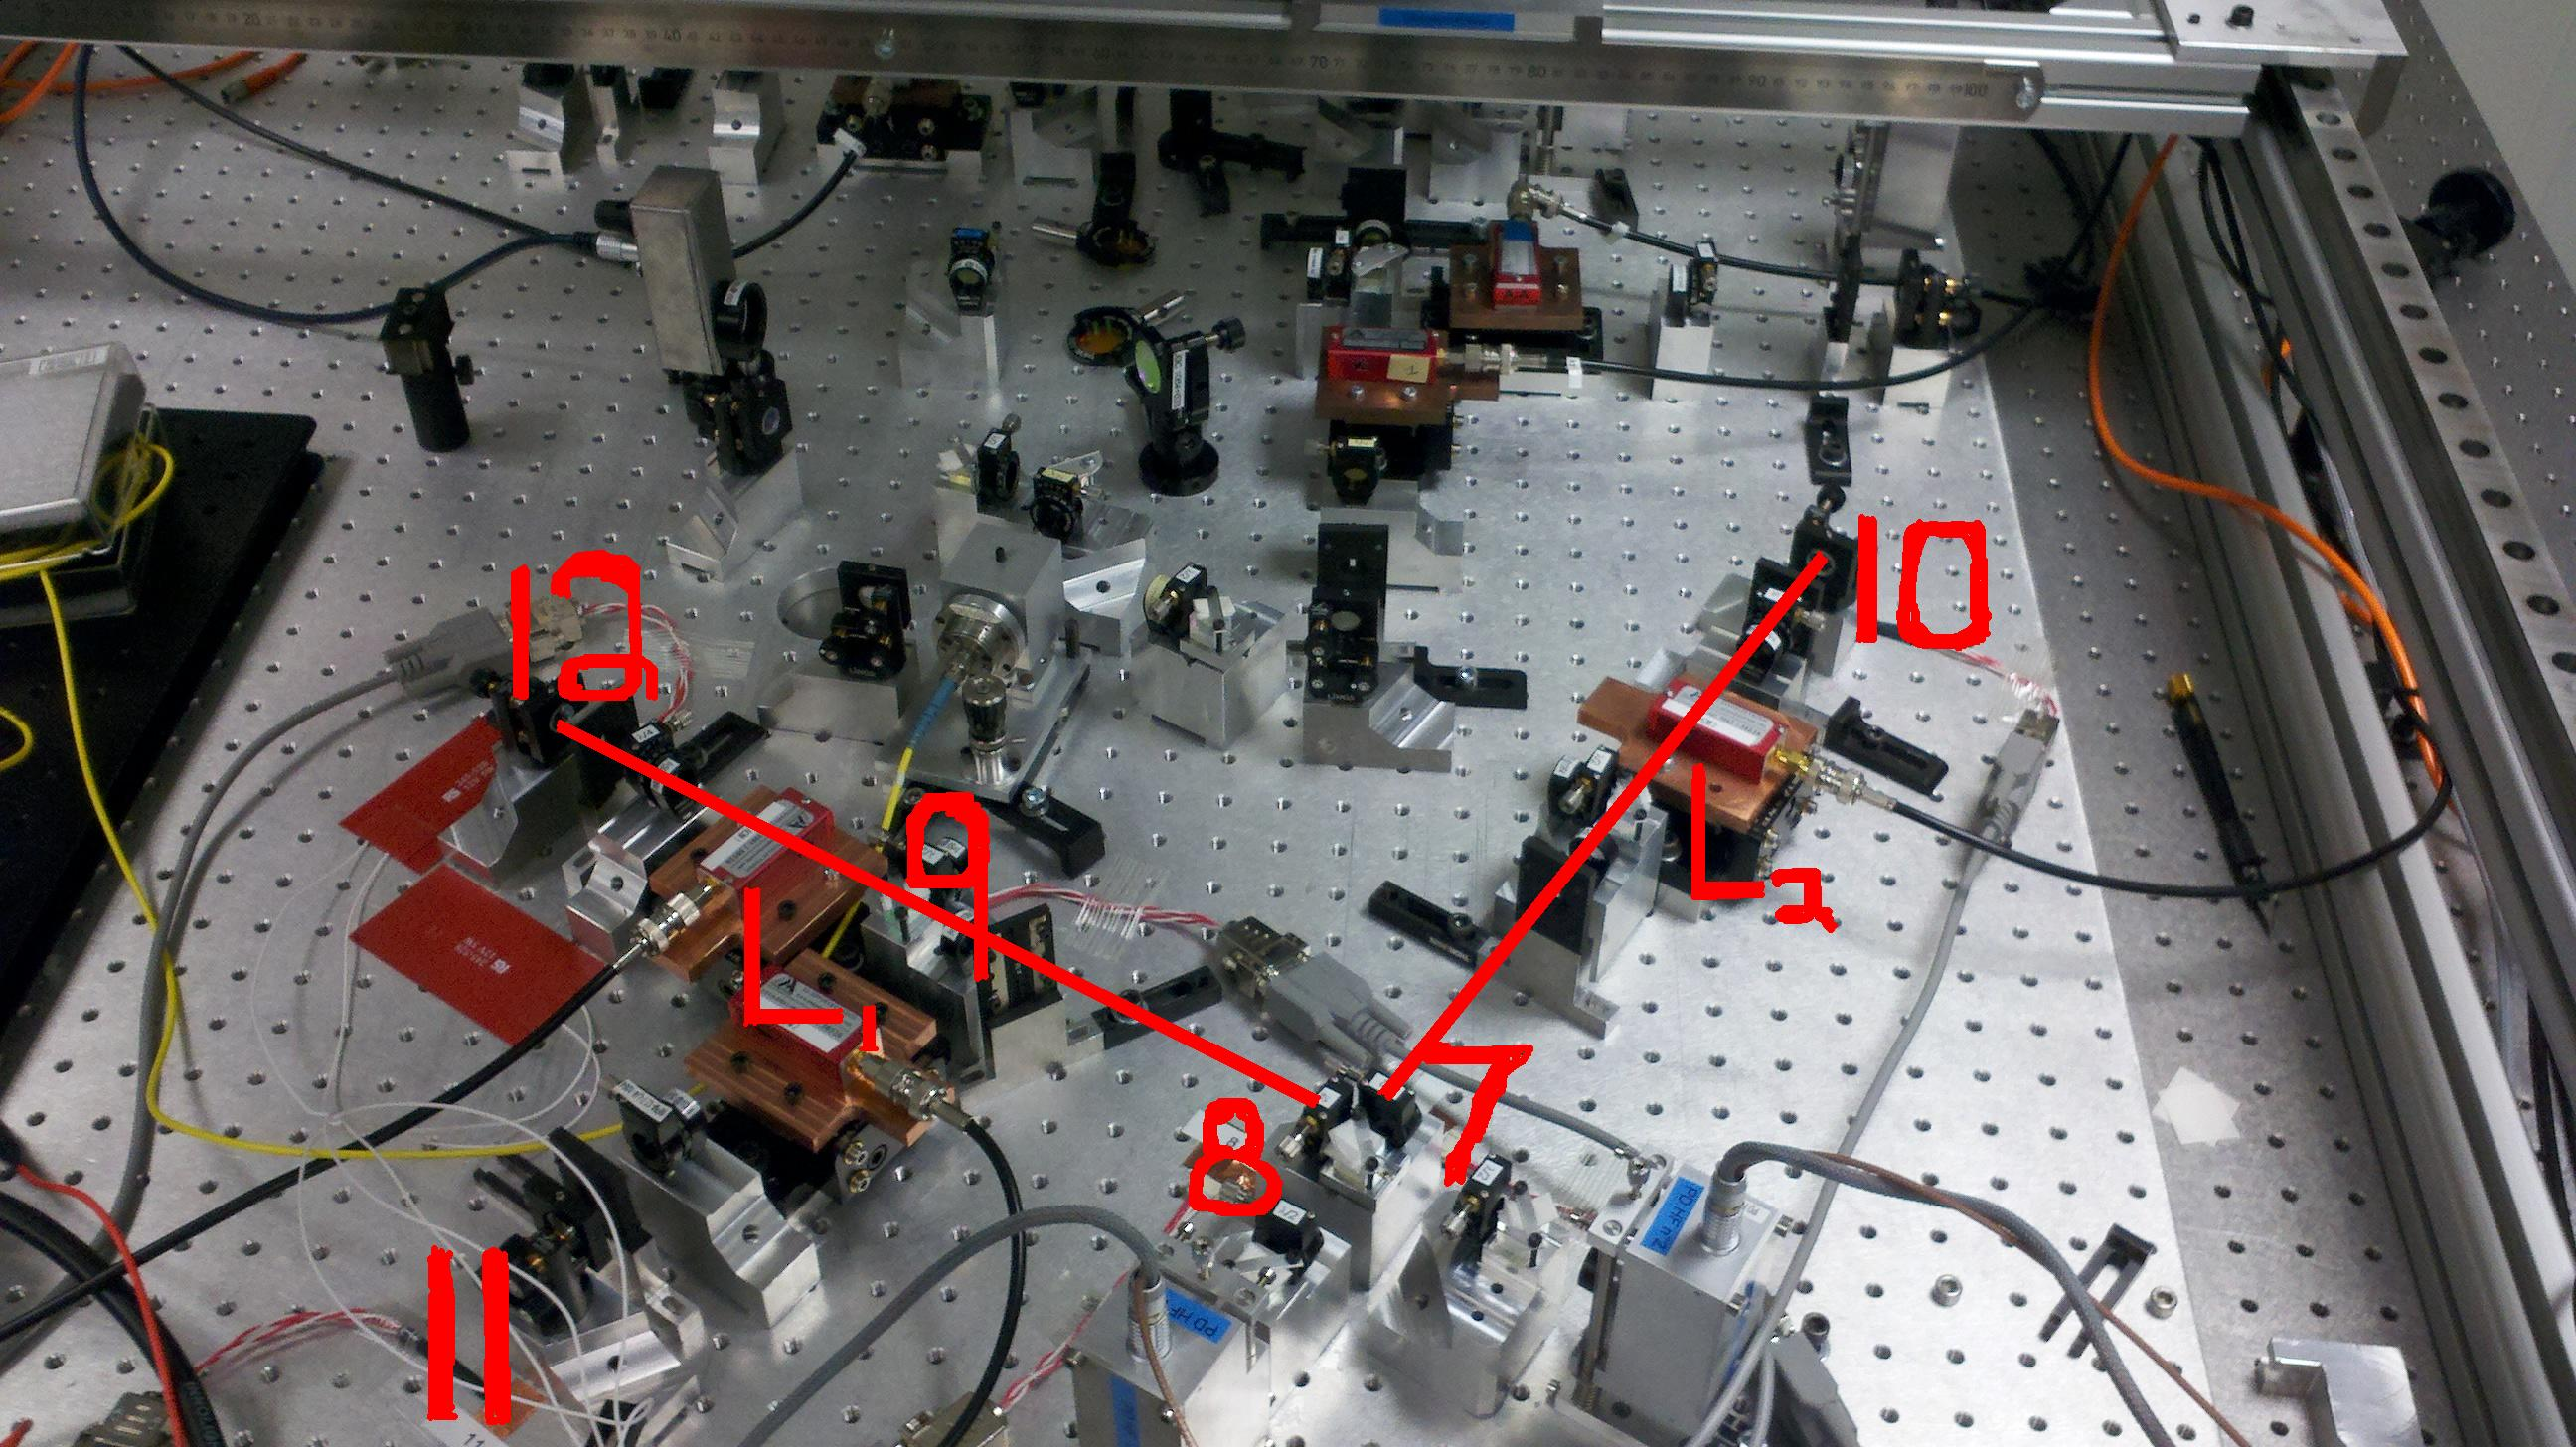
\includegraphics[width=3.64in]{expectations.jpg}\end{center}
%We expect that thermal expansion affecting arm $L_1$ will be caused by variation between $\{T_9, T_{11}, T_{12}\}$ and $\{T_7,T_8\}$, while variation between  $T_{10}$ and $\{T_7,T_8\}$ will affect arm $L_2$, such that
$$\delta L_1 \propto \left\{\begin{array}{l} T_9 \\T_{11} \\T_{12}\end{array}\right. - \left\{\begin{array}{l} T_7 \\T_8 \end{array}\right.\hspace{.5cm}\text{and}\hspace{.5cm} \delta L_2 \propto T_{10} - \left\{\begin{array}{l} T_7 \\T_8 \end{array}\right..$$
%We expect the phase noise to be proportional to the difference in variation along the two arms, such that 
$$\delta\varphi\propto\delta L_1-\delta L_2$$.\\

\end{frame}



\begin{frame}
\frametitle{First Attempt}

\begin{center}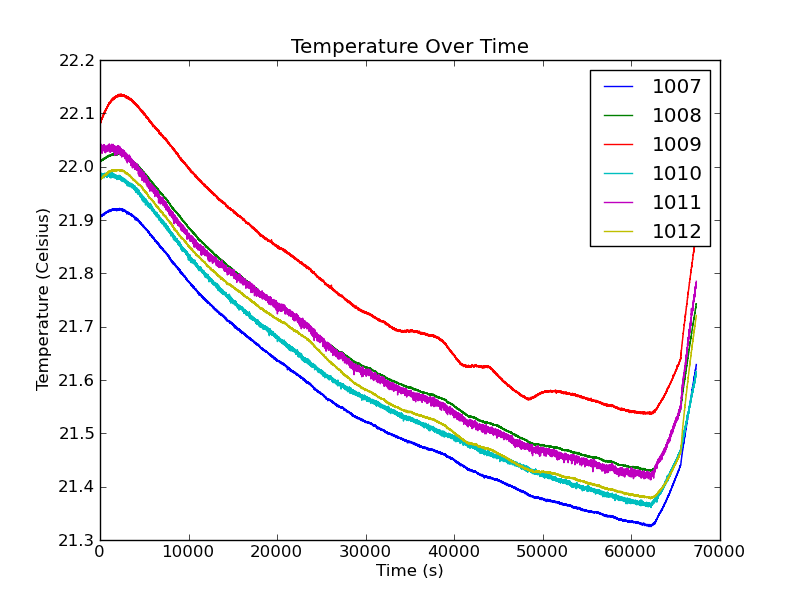
\includegraphics[width=2in]{Figure2.png}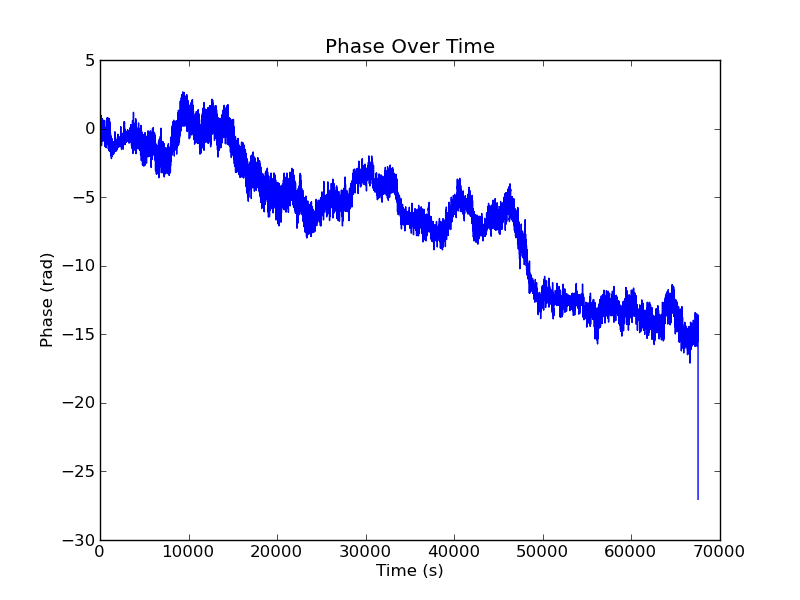
\includegraphics[width=2in]{Figure3.png}\end{center}
\begin{center}\noindent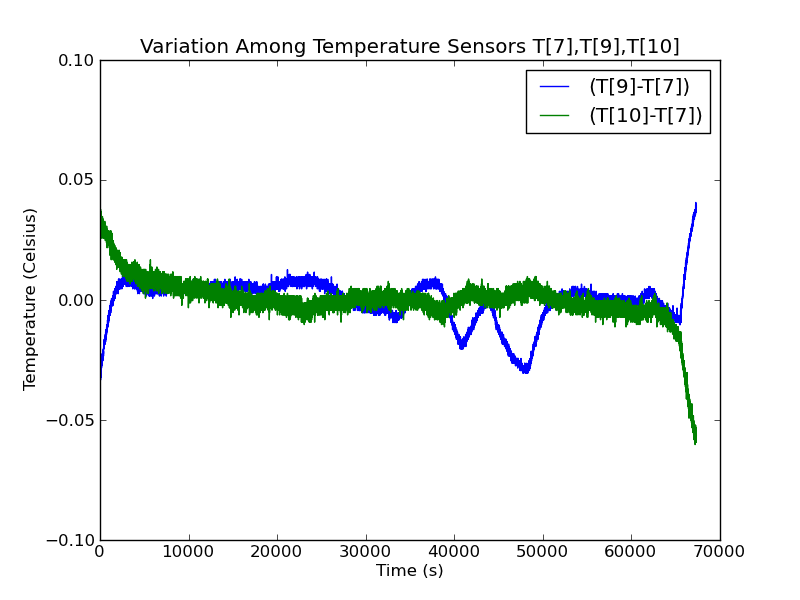
\includegraphics[width=2in]{Tempdiff_7-9-10.png}\end{center}

\end{frame}



\begin{frame}
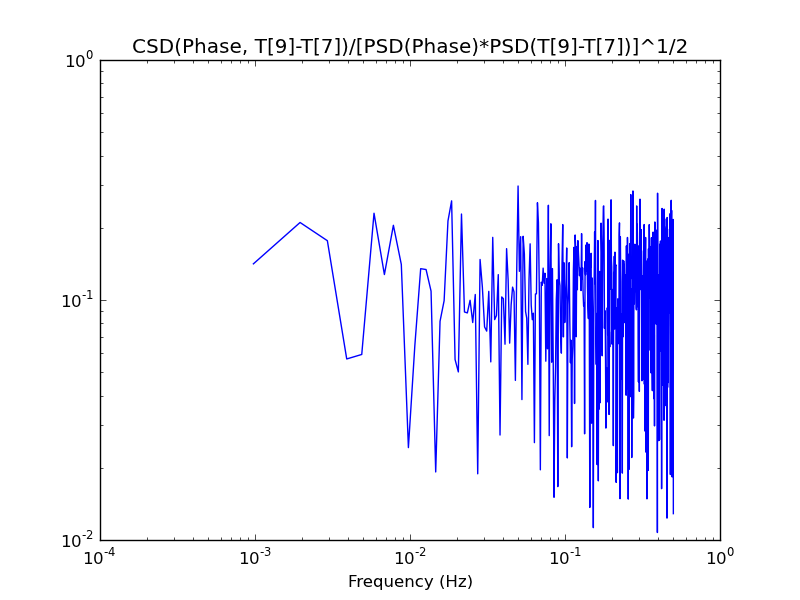
\includegraphics[width=2in]{CSD_phase_9-7_PSD.png}
\end{frame}




\begin{frame}
\frametitle{Lessen Air Turbulence and Modulate Temperature}

\begin{itemize}
\item{Air turbulence is a large source of noise which may mask the temperature noise.}
\item{It will be easier to find correlation if we can modulate the temperature and look for predetermined frequency of phase.}
\end{itemize}
\begin{center}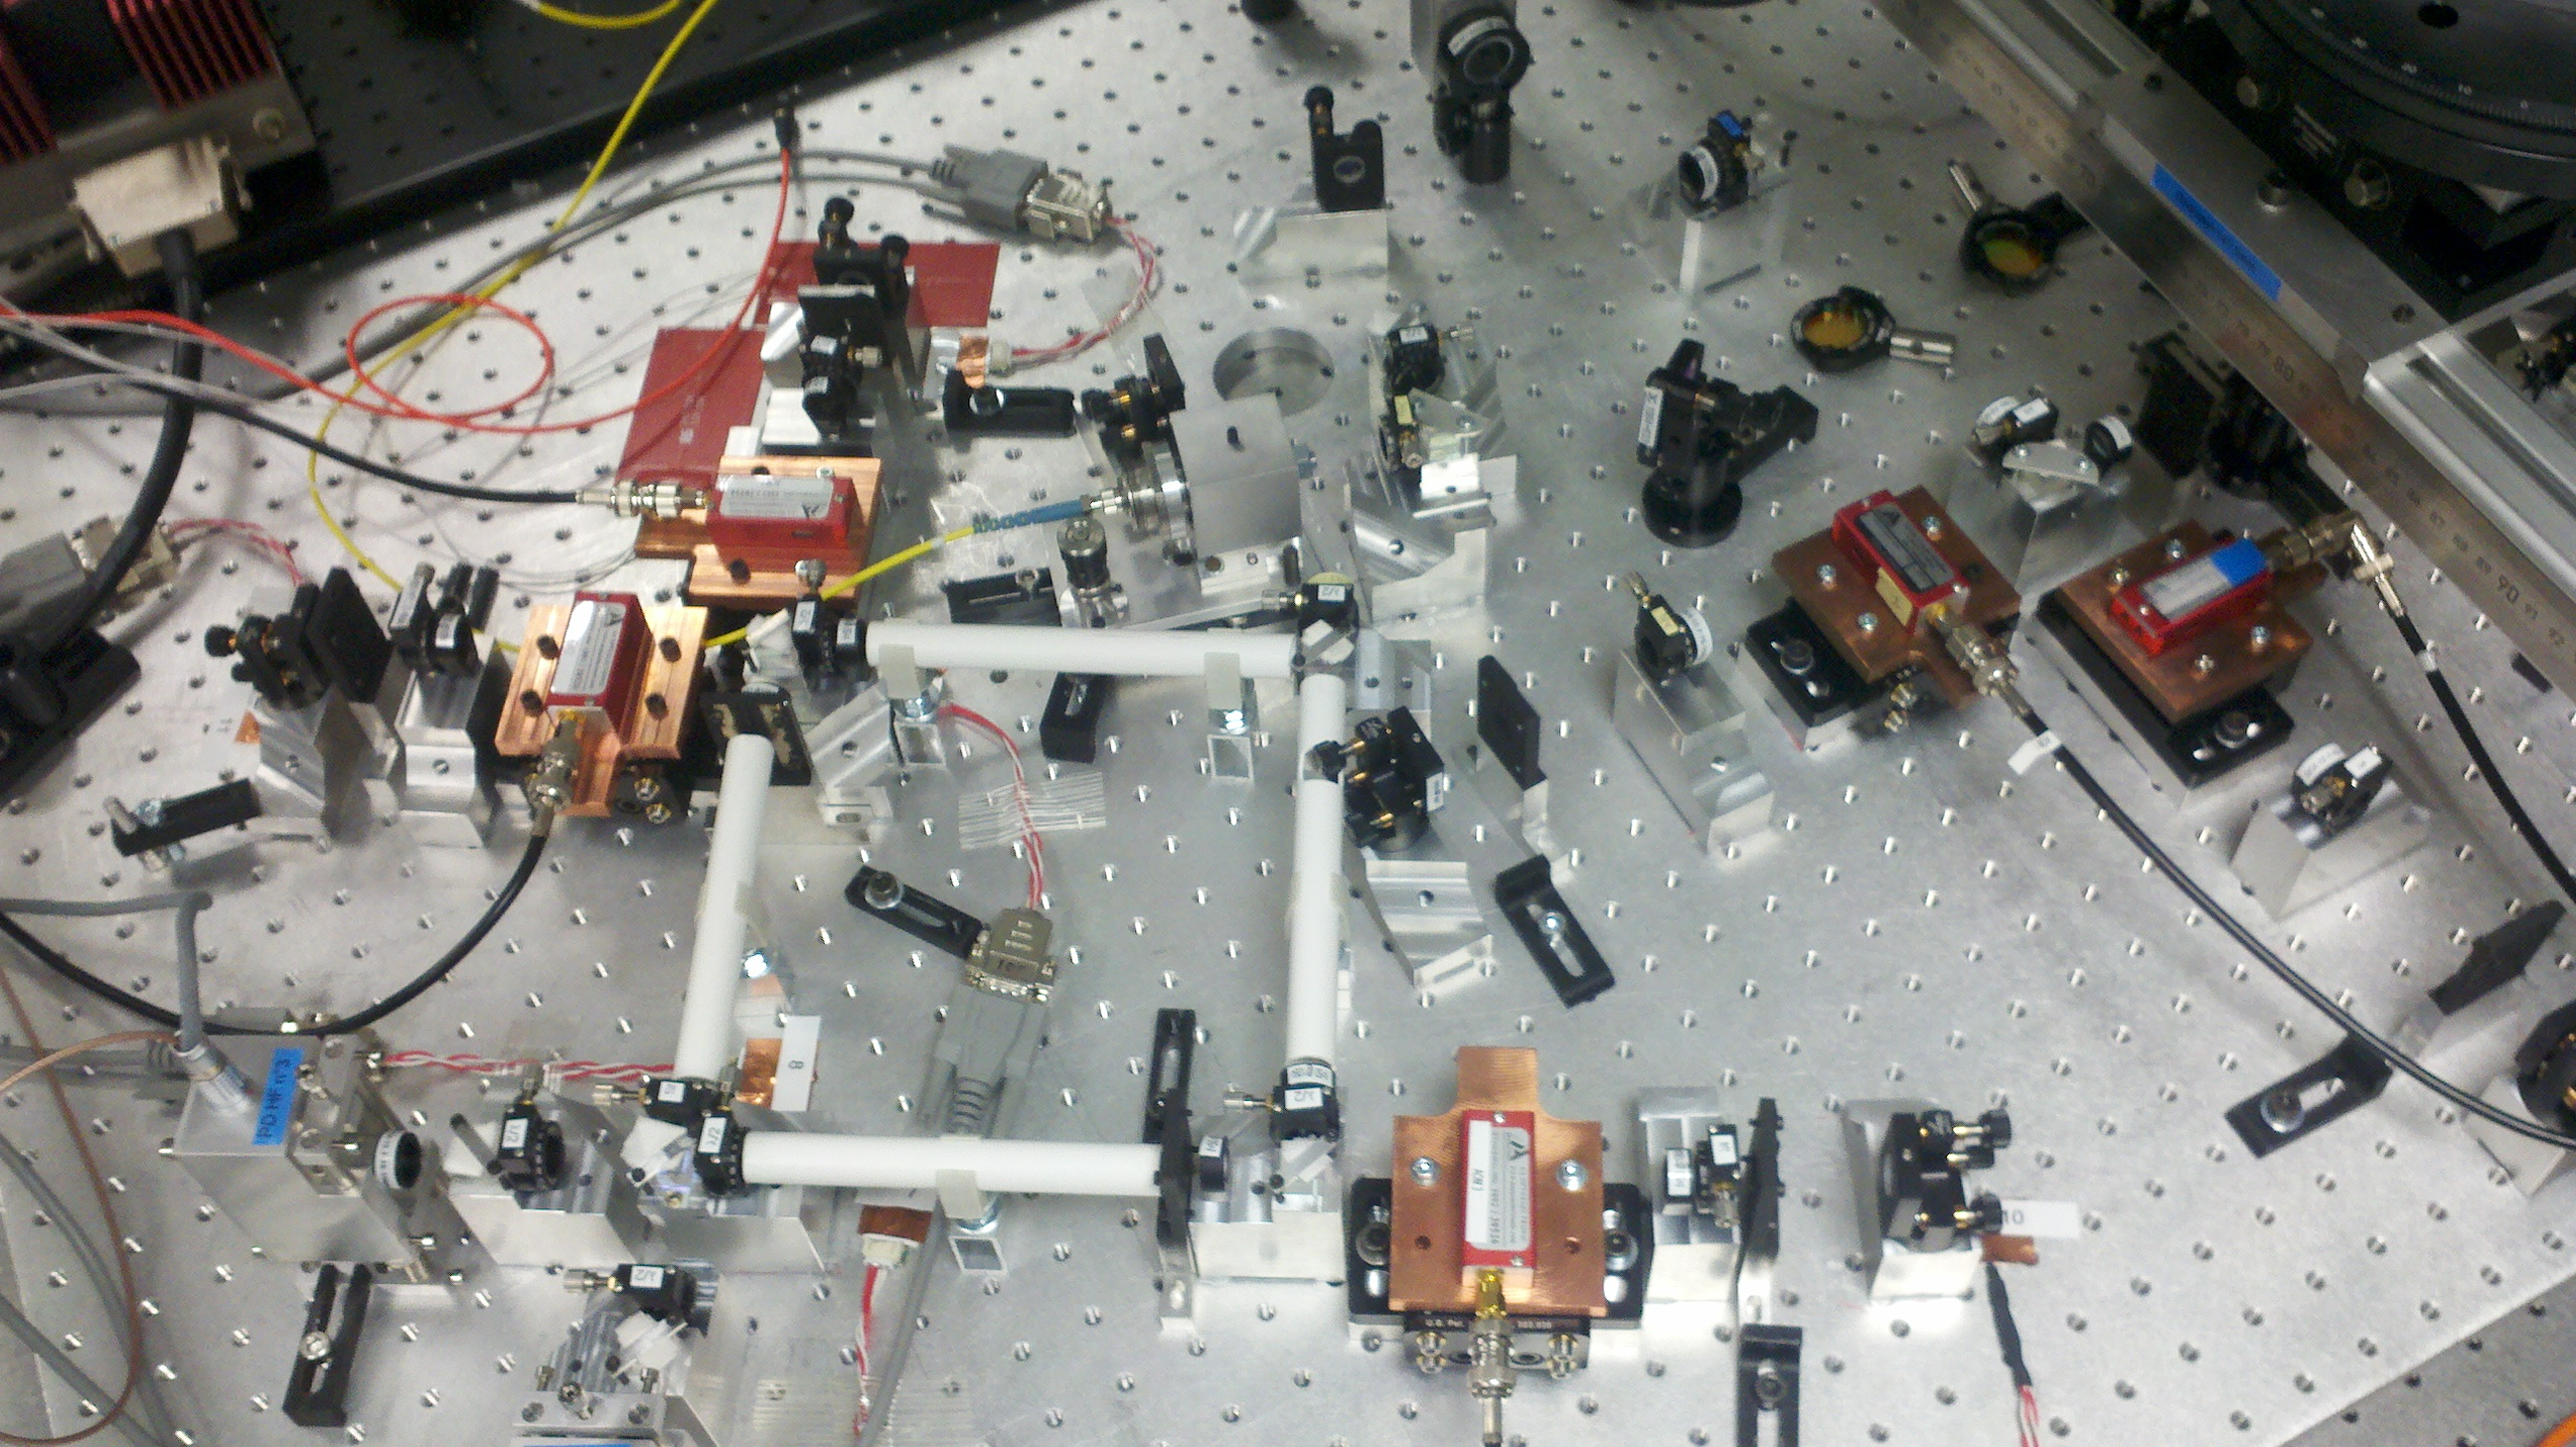
\includegraphics[width=3.4in]{improvements.jpg}\end{center}

\end{frame}



\begin{frame}
\frametitle{Results}

\begin{center}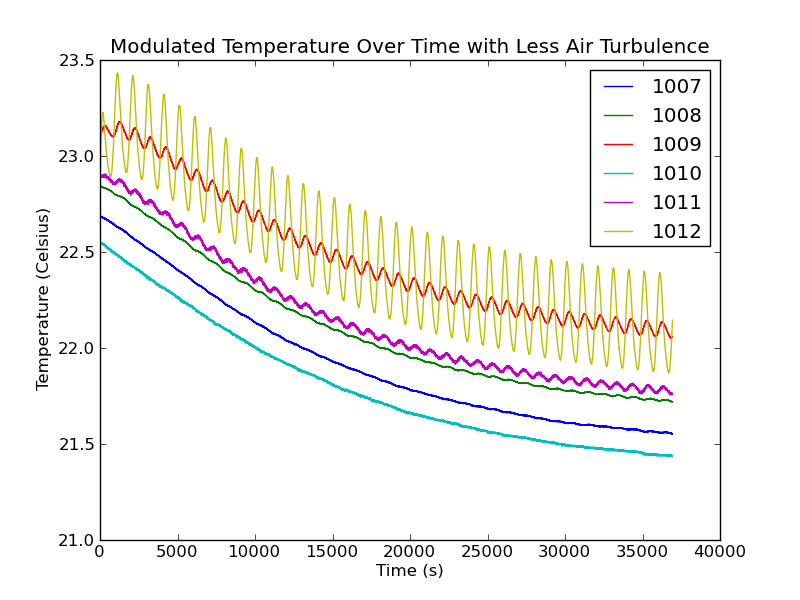
\includegraphics[width=2.03in]{ModulatedTemp.png}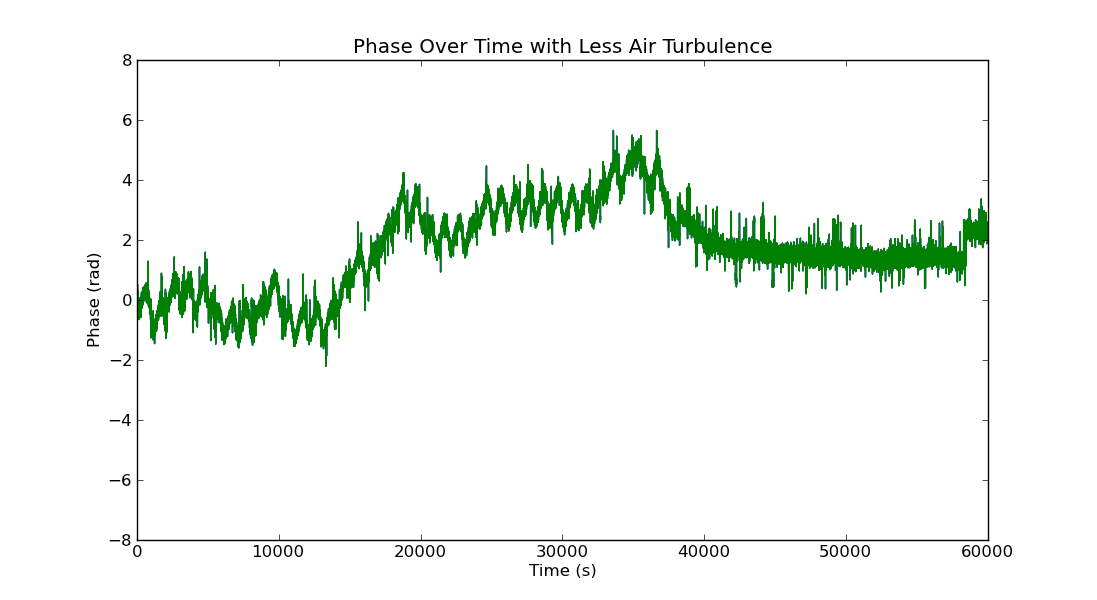
\includegraphics[width=2.5in]{phase260711.png}\\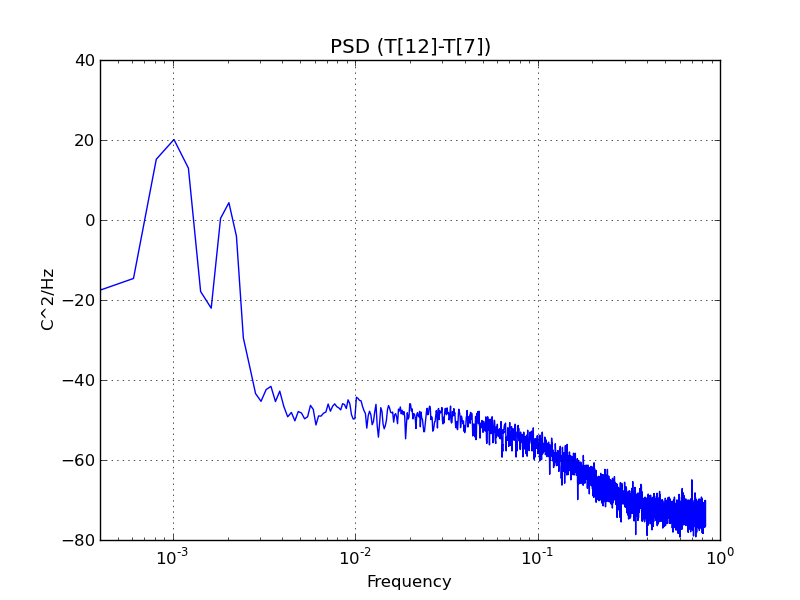
\includegraphics[width=2.1in]{PSD_mod12-7.png}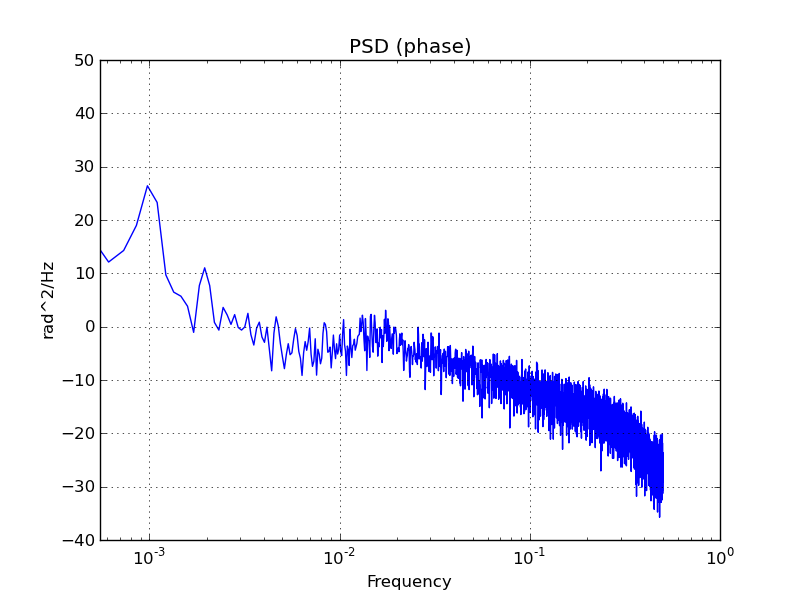
\includegraphics[width=2.1in]{PSD_phasemod.png}\end{center}

\end{frame}



\begin{frame}
\frametitle{Results}

\begin{center}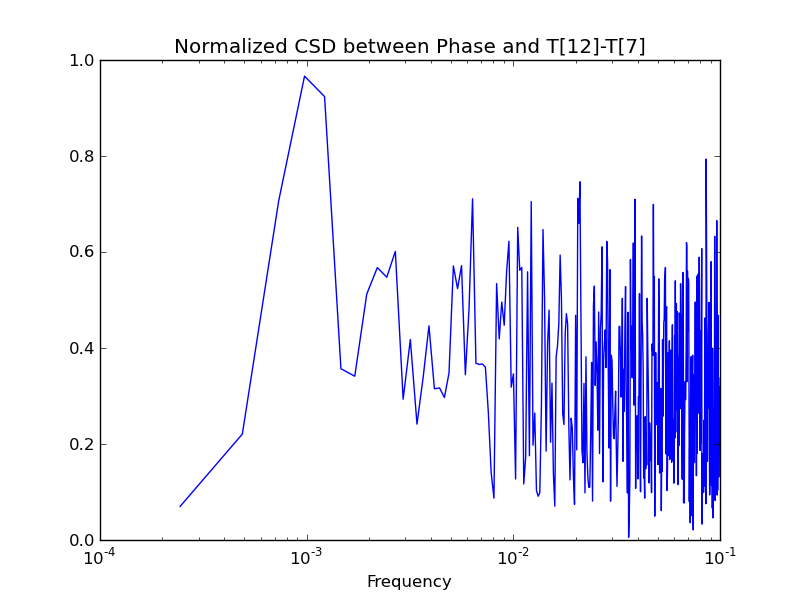
\includegraphics[width=3in]{csd_modphasetemp.png}\end{center}

We have almost perfect correlation at the expected frequency.\\

\end{frame}



\begin{frame}
\frametitle{Conclusion}

This information is very valuable to the experiment. In particular, this creates a greater incentive to mount LOT on an invar plate as opposed to the current aluminum plate.\\
\vspace{.3cm}

Future goals:
\begin{itemize}
\item{Determine correlation relation - allowing us to know the required minimal temperature variation needed to achieve a threshold of phase noise.}
\item{If invar cannot be purchased, find a way to account for the temperature variation in phase data.}
\end{itemize}

\end{frame}



\begin{frame}
\frametitle{Resources}
\begin{itemize}
\item [1] Hubert Halloin et al., "Overview of the LISA Mission and R\&D Developments at the APC", \textit{SF2A 2009}.
\item [2] Hubert Halloin et al., "LISA on Table: An Optical Simulator for LISA", \textit{ICSO 2010}.
\item [3] "Laser Interferometer Space Antenna", \textit{http://en.wikipedia.org/wiki/Laser\_Interferometer\_Space\_Antenna''}.
\end{itemize}

\end{frame}
%%%%%


\end{document}